\documentclass[../resumosRCOM.tex]{subfiles}
 
\begin{document} 

\subsubsection{Graphs}

\paragraph{Directed:}

\begin{center}
    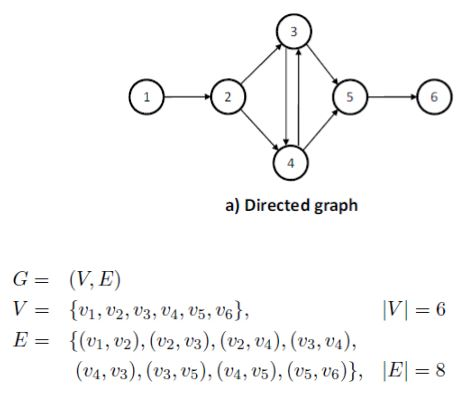
\includegraphics[scale=0.5]{directed}
\end{center}

\paragraph{Undirected:}

\begin{center}
    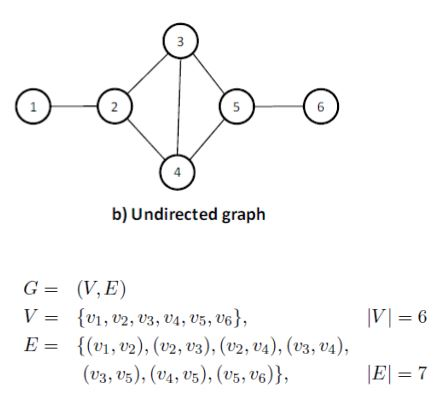
\includegraphics[scale=0.5]{undirected}
\end{center}

\subsubsection{Tree}

\begin{itemize}
    \item Tree T = (V,E)
    \begin{itemize}
        \item Graph with no cycles
        \item |E| = |V| - 1
        \item Any two V connected by only one E
    \end{itemize}
    \item A tree T spans a graph G = (V,E) (spanning tree) if
    \begin{itemize}
        \item T = (V,E') \& E $\subseteq$ E' (T must have the same vertices and a subset of the graph edges)
    \end{itemize}
\end{itemize}

\begin{center}
    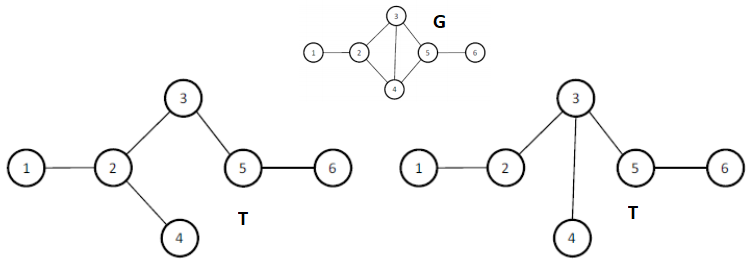
\includegraphics[scale=0.5]{tree}
\end{center}

\subsubsection{Shortest Path Trees}

\begin{itemize}
    \item Graphs and Trees can be weighted
    \begin{itemize}
        \item G=(V,E,W)
        \item T=(V,E',W)
    \end{itemize}
    \begin{center}
        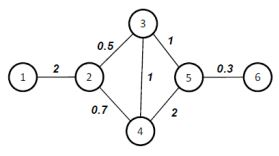
\includegraphics[scale=0.75]{weighted}
    \end{center}
    \item Total cost of a tree T \[C_{total}(T) = \sum_{i=1}^{|E|}\] (sum of all tree edges weight)
    \item Minimum spanning tree T$^*$ \[C_{total}(T^*) = min(C_{total}(T))\]
    \begin{itemize}
        \item algorithms used to compute MST: Prism, Kruskal
    \end{itemize}
    \item \textbf{Shortest Path Tree (SPT) rooted at vertex} s
    \begin{itemize}
        \item tree composed by the \textbf{union of the shortest paths between} s \textbf{and each vertex of} G
        \item algorithms used to compute SPT: \textbf{Dijkstra}, \textbf{Bellman-Ford}
    \end{itemize}
    \item Computer networks use \textbf{Shortest Path Trees}
\end{itemize}

\subsection{Routing in Layer 3 Networks}

\subsubsection{Forwarding, Routing}

\begin{itemize}
    \item \textbf{Forwarding} $\rightarrow$ data plane
    \begin{itemize}
        \item directing packet from input to output link
        \item using a forwarding table
    \end{itemize}
    \item \textbf{Routing} $\rightarrow$ control plane
    \begin{itemize}
        \item computing paths the packets will follow
        \item routers exchange messages
        \item each router creates its forwarding table
    \end{itemize}
\end{itemize}

\subsubsection{Importance of Routing}

\begin{itemize}
    \item End-to-end performance
    \begin{itemize}
        \item path affects quality of service
        \item delay, throughput, packet loss
    \end{itemize}
    \item Use of network resources
    \begin{itemize}
        \item balance traffic over routers and links
        \item avoiding congestion by directing traffic to less-loaded links
    \end{itemize}
    \item Transient disruptions
    \begin{itemize}
        \item failures, maintenance
        \item limiting packet loss and delay during changes
    \end{itemize}
\end{itemize}

\subsubsection{Shortest-Path Routing}

\paragraph{Path-selection model}

\begin{itemize}
    \item Destination-based
    \item Load-insensitive (ex: static link weights)
    \item Minimum hop count or minimum sum of link weights
\end{itemize}

\begin{center}
    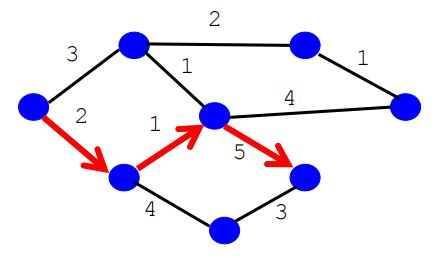
\includegraphics[scale=0.5]{SPR}
\end{center}

\subsubsection{Shortest-Path Problem}

\begin{itemize}
    \item Given a network topology with link costs
    \begin{itemize}
        \item \textbf{c(x,y)} - link cost from node x to node y
        \item $\infty$ if x and y are not direct neighbors
    \end{itemize}
    \item Compute the least-cost paths from source \textbf{u} to all nodes
    \begin{itemize}
        \item \textbf{p(v)} - node predecessor of node v in the path from u
    \end{itemize}
\end{itemize}

\begin{center}
    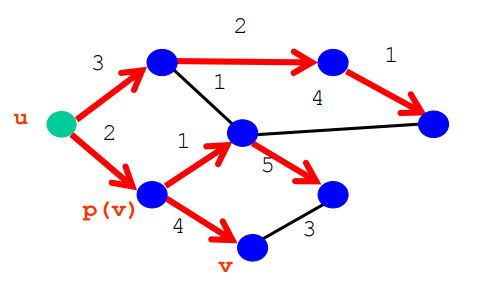
\includegraphics[scale=0.5]{SPP}
\end{center}

\subsubsection{Dijkstra’s Shortest-Path Algorithm}

\begin{itemize}
    \item Iterative algorithm
    \begin{itemize}
        \item After k iterations $\rightarrow$ known least-cost paths to k nodes
    \end{itemize}
    \item \textbf{S} $\rightarrow$ set of nodes for which least-cost path is known
    \begin{itemize}
        \item Initially, \textbf{S=\{u\}}, where \textbf{u} is the source node
        \item Add one node to \textbf{S} in each iteration
    \end{itemize}
    \item \textbf{D(v)} $\rightarrow$ current cost of path from source to node \textbf{v}
    \begin{itemize}
        \item Initially
        \begin{itemize}
            \item \textbf{D(v)=c(u,v)} for all nodes adjacent to \textbf{u}
            \item \textbf{D(v)=$\infty$} for all other nodes \textbf{v}
        \end{itemize}
        \item Continually update \textbf{D(v)} when shorter paths are learned
    \end{itemize}
\end{itemize}

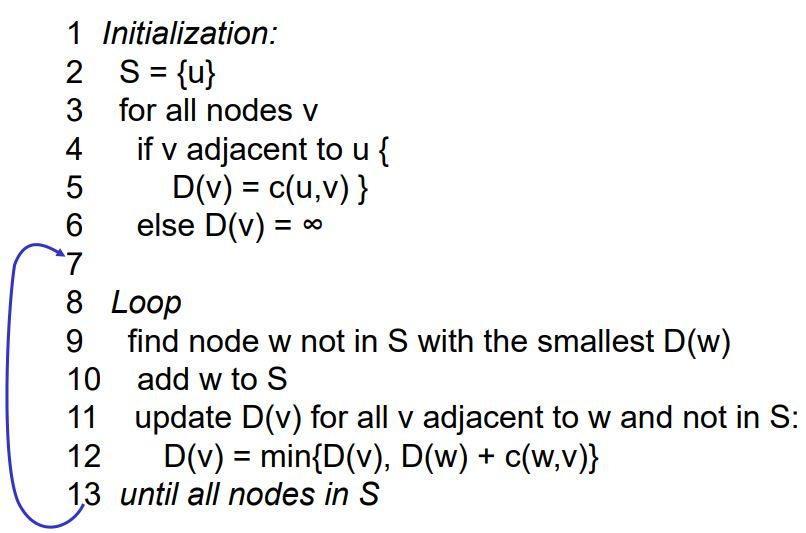
\includegraphics[scale = 0.5]{Dijkstra}

\subsubsection{Shortest-Path Tree}

\begin{itemize}
    \item Shortest-path tree from u
    \begin{center}
        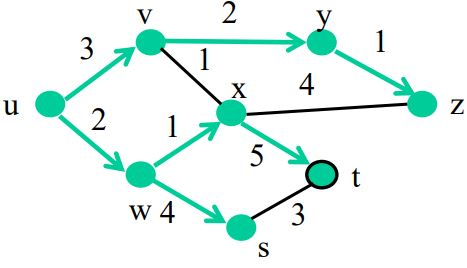
\includegraphics[scale=0.5]{SPT}
    \end{center}
    \item Forwarding table at u
    \begin{center}
        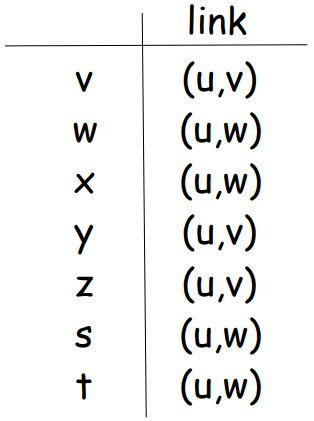
\includegraphics[scale=0.5]{FT(u)}
    \end{center}
\end{itemize}

\subsubsection{Link-State Routing}

\begin{itemize}
    \item Each router keeps track of its incident links
    \begin{itemize}
        \item link up, link down
        \item cost on the link
    \end{itemize}
    \item Each router broadcasts link state
    \begin{itemize}
        \item every router gets a complete view of the graph
    \end{itemize}
    \item \textbf{Each router runs Dijkstra’s algorithm}, to
    \begin{itemize}
        \item compute the shortest paths
        \item construct the forwarding table
    \end{itemize}
\end{itemize}

\subsubsection{Detection of Topology Changes}

\begin{itemize}
    \item Beacons generated by routers on links
    \begin{itemize}
        \item periodic “hello” messages in both directions
        \item few missed “hellos” $\rightarrow$ link failure
    \end{itemize}
\end{itemize}

\subsubsection{Broadcasting the Link State}

\begin{itemize}
    \item How to Flood the link state?
    \begin{itemize}
        \item every node sends link-state information through adjacent links
        \item next nodes forward that info to all links except the one where the information arrived
    \end{itemize}
    \begin{center}
        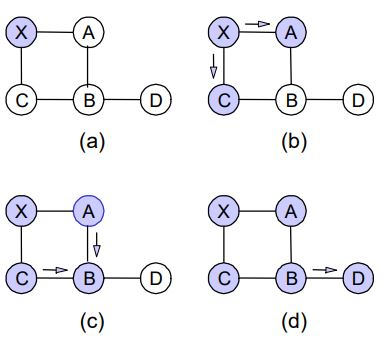
\includegraphics[scale=0.5]{BLS}
    \end{center}
    \item When to initiate flooding?
    \begin{itemize}
        \item Topology change
        \begin{itemize}
            \item link or node failure/recovery
            \item link cost change
        \end{itemize}
    \end{itemize}
    \begin{itemize}
        \item Periodically
        \begin{itemize}
            \item refresh link-state information
            \item typically 30 minutes
        \end{itemize}
    \end{itemize}
\end{itemize}

\subsubsection{Scaling Link-State Routing}

\begin{itemize}
    \item Overhead of link-state routing
    \begin{itemize}
        \item flooding link-state packets throughout the network
        \item running Dijkstra’s shortest-path algorithm
    \end{itemize}
    \item Introducing hierarchy through “areas”
\end{itemize}

\begin{center}
    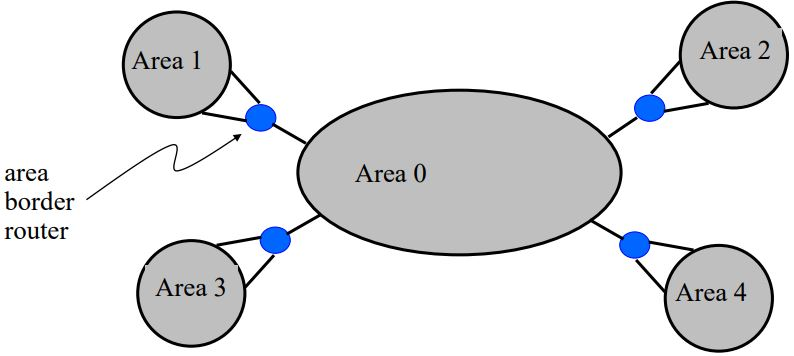
\includegraphics[scale=0.5]{areas}
\end{center}

\subsubsection{Bellman-Ford Algorithm}

\begin{itemize}
    \item Define distances at each node x
    \begin{itemize}
        \item d$_x$(y) = cost of least-cost path from x to y
    \end{itemize}
    \item Update distances based on neighbors
    \begin{itemize}
        \item d$_x$(y) = min \{c(x,v) + $d_v(y)$\} over all neighbors v
    \end{itemize}
\end{itemize}

\begin{center}
    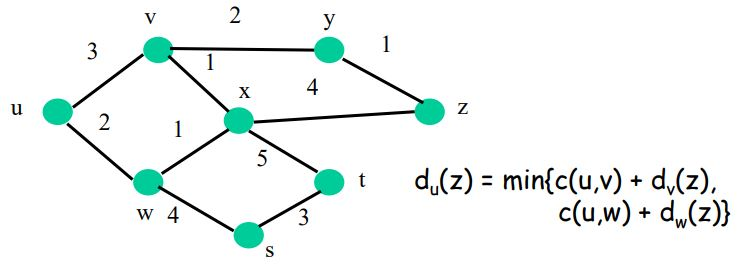
\includegraphics[scale=0.5]{BF}
\end{center}

\subsubsection{Distance Vector Algorithm}

\begin{itemize}
    \item c(x,v) = cost for direct link from x to v
    \begin{itemize}
        \item node x maintains costs of direct links \textbf{c(x,v)}
    \end{itemize}
    \item D$_x$(y) = estimate of least cost from x to y
    \begin{itemize}
        \item node x maintains distance vector \textbf{D$_x$ = [D$_x$(y): y $\in$ N ]}
    \end{itemize}
    \item Node x maintains also its neighbors’ distance vectors
    \begin{itemize}
        \item for each neighbor v, x maintains \textbf{D$_v$ = [D$_v$(y): y $\in$ N ]}
    \end{itemize}
    \item Each node v periodically sends D$_v$ to its neighbors
    \begin{itemize}
        \item and neighbors update their own distance vectors
        \item D$_x$(y) $\leftarrow$ min$_v$\{c(x,v) + D$_v$(y)\} for each node y $\in$ N
    \end{itemize}
    \item Over time, the distance vector D$_x$ converges
\end{itemize}

\begin{itemize}
    \item Iterative, asynchronous, each local iteration caused by:
    \begin{itemize}
        \item local link cost change 
        \item distance vector update message from neighbor
    \end{itemize}
    \item Distributed
    \begin{itemize}
        \item node notifies neighbors only when its DV changes
    \end{itemize}
    \item Neighbors then notify their neighbors, if necessary
\end{itemize}

\begin{center}
    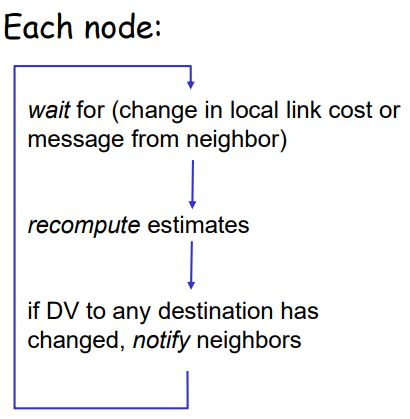
\includegraphics[scale=0.5]{DVA}    
\end{center}

\subsubsection{Routing Information Protocol (RIP)}

\begin{itemize}
    \item Distance vector protocol
    \begin{itemize}
        \item nodes send distance vectors every 30 seconds
        \item or when an update causes a change in routing
    \end{itemize}
    \item RIP is limited to small networks
\end{itemize}

\subsubsection{BGP – The Exterior Gateway Routing Protocol}

\begin{center}
    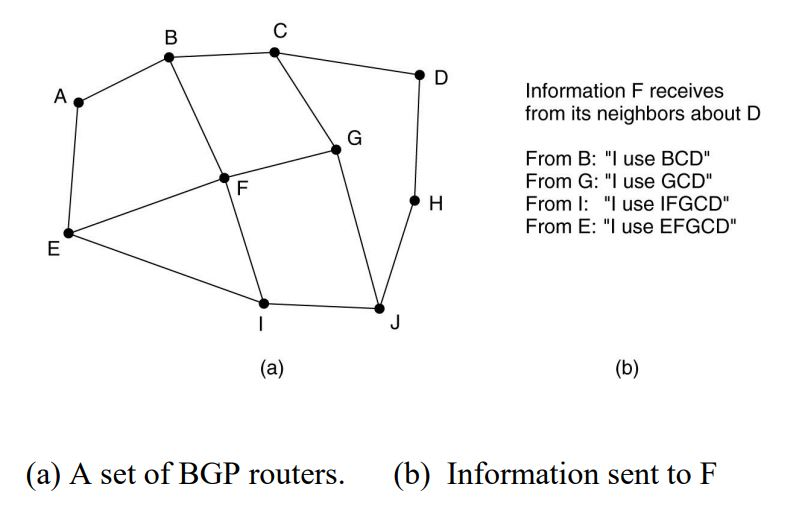
\includegraphics[scale=0.5]{BGP}
\end{center}

\subsection{Unique Spanning Tree in Ethernet Networks}

\subsubsection{L2 Networking - Single Tree Required}

\begin{itemize}
    \item Ethernet frame
    \begin{itemize}
        \item No hop-count
        \item Could loop forever
        \item broadcast frame, mis-configuration
    \end{itemize}
    \begin{center}
        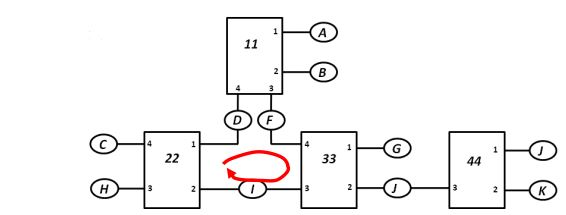
\includegraphics[scale=0.5]{loop}
    \end{center}
    \item Layer 2 network
    \begin{itemize}
        \item \textbf{Required to have tree topology}
        \item Single path between every pair of stations
    \end{itemize}
    \item Spanning Tree Protocol (STP)
    \begin{itemize}
        \item Running in bridges
        \item Helps building the spanning tree
        \item Blocks ports
    \end{itemize}
    \begin{center}
        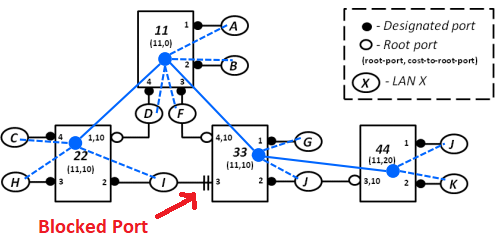
\includegraphics[scale=0.5]{STP}
    \end{center}
\end{itemize}

\subsubsection{Constructing a Spanning Tree}

\begin{itemize}
    \item Distributed algorithm
    \begin{itemize}
        \item switches need to elect a “root”
        \begin{itemize}
            \item the switch with the smallest identifier
        \end{itemize}
        \item each switch identifies if its interface is on \textbf{the shortest path from the root}
        \item messages(Y,d,X)
        \begin{itemize}
            \item from node X
            \item claiming Y is the root
            \item and the distance is d
        \end{itemize}
    \end{itemize}
\end{itemize}

\begin{center}
    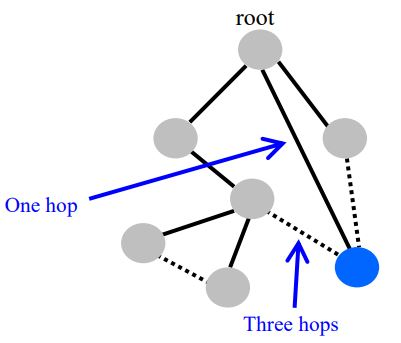
\includegraphics[scale=0.5]{CST}
\end{center}

\subsubsection{Steps in Spanning Tree Algorithm}

\begin{itemize}
    \item Initially, each switch thinks it is the root
    \begin{itemize}
        \item switch sends a message out every interface
        \item identifying itself as the root with distance 0
    \end{itemize}
    \item Other switches update their view of the root
    \begin{itemize}
        \item upon receiving a message, check the root id
        \item if the new id is smaller, start viewing that switch as root
    \end{itemize}
    \item Switches compute their distance from the root
    \begin{itemize}
        \item add 1 to the distance received from a neighbor
        \item identify interfaces not on a shortest path to the root and exclude them from the spanning tree
    \end{itemize}
\end{itemize}

\subsection{Maximum Flow of a Network}

\subsubsection{Flow Network Model}

\begin{itemize}
    \item \textbf{Flow network}
    \begin{itemize}
        \item source s
        \item sink t
        \item nodes a, b and c
    \end{itemize}
    \item Edges are labeled with \textbf{capacities (ex: bit/s)}
    \begin{center}
        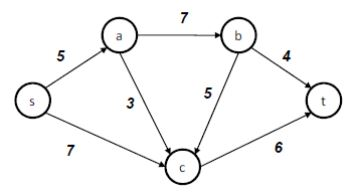
\includegraphics[scale=0.5]{FNM}
    \end{center}
    \item Communication networks are not flow networks
    \begin{itemize}
        \item they are queue networks
        \item flow networks enable to determine limit values
    \end{itemize}
\end{itemize}

\subsubsection{Maximum Capacity of a Flow Network}

\begin{itemize}
    \item Max-flow min-cut theorem
    \begin{itemize}
        \item maximum amount of flow transferable through a network
        \item equals minimum value among all simple cuts of the network
    \end{itemize}
    \item Cut $\rightarrow$ split of the nodes V into two disjoint sets S and T
    \begin{itemize}
        \item $S \cup T = V$
        \item there are $2^{|V|-2}$ possible cuts
    \end{itemize}
    \item Capacity of cut (S,T): \[c(S,T)=\sum_{(u,v) | u\in S,v\in T,(u,v)\in E}c(u,v)\]
    \begin{itemize}
        \item (sum of the cost of all edges from S to T)
    \end{itemize}
\end{itemize}

\end{document}